\documentclass[]{article}
\usepackage{graphicx}

%opening
\title{Note on GMM Estimation of Theories of Expectation Formation}
\author{Tao Wang}

\begin{document}

\maketitle

\section{Generic Framework}


\section{Estimation}
\subsection{Real-Time Data}

\begin{figure}
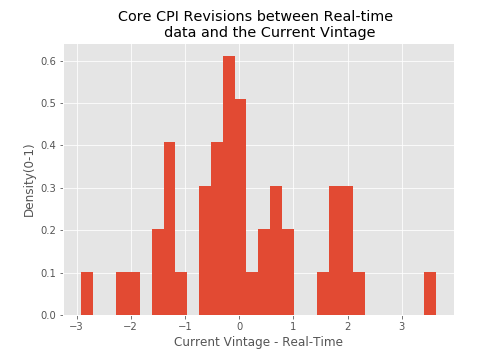
\includegraphics[width=\textwidth]{figures/hist_rev_realtime.png}
\caption{Revisions of Current-vintage from Real-time Core CPI}
\label{real_time_rev}
	\begin{flushleft}
	{\footnotesize Note: real-time data  at time $t$ is defined the inflation from $t-1$ to $t$ according to the most recent vintage of CPI inflation at time $t$. The period is between 2000 M1-2018 M3.}
\end{flushleft}
\end{figure}


\begin{figure}
	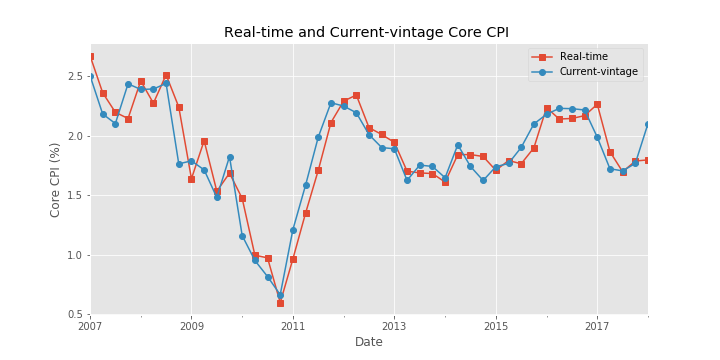
\includegraphics[width=\textwidth]{figures/ts_rev_realtime.png}
	\caption{Current-vintage and Real-time Core CPI}
	\label{ts_real_time_current_vintage}
\end{figure}

\subsection{Results}

\end{document}
